\documentclass[master.tex]{subfiles}
 
\newcommand{\meanxy}[1]{\left<#1\right>_{z,y}}
\newcommand{\Tflow}[0]{\overline{\Gamma}}

\begin{document}



\chapter{Effect of Polarization Equation Linearizations on tokamak edge turbulence}\label{sec:polarization_equation_evaluation}

\section{Introduction}
In both gyrokinetic and gyrofluid models the polarization equation plays a central role and the nonlinear nature is often approximated because of the large computational effort associated with the numerical schemes and the assumption that the amplitudes of turbulent fluctuations are much smaller than the background. This may hold for the core plasma but certainly not for the edge region where high background gradients are observed which lead to relatively high amplitude fluctuations if dense \textit{material} is transported from the core region of the separatrix into the \ac{SOL}. For instance the GYSELA polarization equation assumes a equilibrium density $n_0(r)$ where $r$ is to be identified with the $x$-direction \cite{GYSELACODE}. This comes close to linearization 3. The XGC1 code uses a similar approach \cite{XGC1Code}. The GENE code keeps evaluates the non-linearity but claims that it does only have an effect if the electron Debye length $\lambda_{De}$ is comparable to the electron gyro radius $\rho_e$ which in a tokamak is not the case. The following results should give some insight on the effects of the different linearizations. It should be noted that this is not an extensive parameter study and considering the amount of parameters (>10) there could exist various other effects that are not represented by the particular parameters used in the following evaluation.

\section{Simulation Setup}

The evaluation of the linearizations is done on a 8x128x512 8x256x1024 grid with $h_x$ and $h_y=1.0|0.5$ respectively. The following parameter set is used for the smaller grid:
\begin{itemize}
    \item $\Delta t$: 0.025
    \item $\hat{c}$: 5.0
    \item $\hat{\epsilon}$: 27000.0
    \item $mcv$: 0.02
    \item $magnetic Shear$: 1.2
    \item $\nu_{\parallel}$: 0.11
    \item $\nu_{\perp}$: 0.11
    \item core Density: 1.5
    \item edge Density: 0.13
\end{itemize}
The simulation is run on \ac{TV} node using the GPU implementations of the \ac{SOR}-solver and gyroaveraging operator. The lower resolution grid has been run for 400.000 iterations and a state snapshot is taken every 20,000 iterations. Due to time and disk space limitations for the higher resolution only 200.000 iterations are done as well as $\Delta t$ is reduced to $0.01$ to stay in the \ac{CFL} limit.

\section{Equilibrium State}
At first the simulation develops strong turbulence and high fluctuations which result in an outburst of "material" (i. e. the total density decreases). Afterwards the simulation approaches a steady state where the properties only change little. \todo{Place Figure of Energy} This behavior can be seen by looking at the $\mathrm{E} \times \mathrm{B}$-Energy and the total density both restricted to the core-plasma (in/out separatrix). The idea now is to compare mean values over the simulation time where a equilibrium state has been reached. 

The errors attached to the mean values are calculated via the standard derivation but do not represent the error of multiple simulations but rather give an idea about the size of fluctuations in the equilibrium state.

\section{Evaluation}
To compare the different linearizations defined in \autoref{sec:polarization-linearizations} the mean turbulent flow in the steady state regime is compared for the core and \ac{SOL} plasma. Further on the zonal potential  $\meanxy{\phi_e}$, the zonal flow ($\partial_x \meanxy{\phi_e}$) and the vorticity also defined as zonal flow potential ($\partial_{xx}\meanxy{\phi_e}$) are compared and finally the parallel velocity is taken into account.




\section{Turbulent Flow}
The turbulent flow is calculated as it is defined in \autoref{sec:simulation_quantities}. After the simulation has reached a stable regime a mean value is taken and compared. The turbulent flows for the whole simulation are displayed in \autoref{fig:turbulent-flow-low} on a semi logarithmic grid. From this figure one can already see that there is no apparent difference for the turbulent flows in regard to the linearizations.
\begin{figure}[!htbp]
    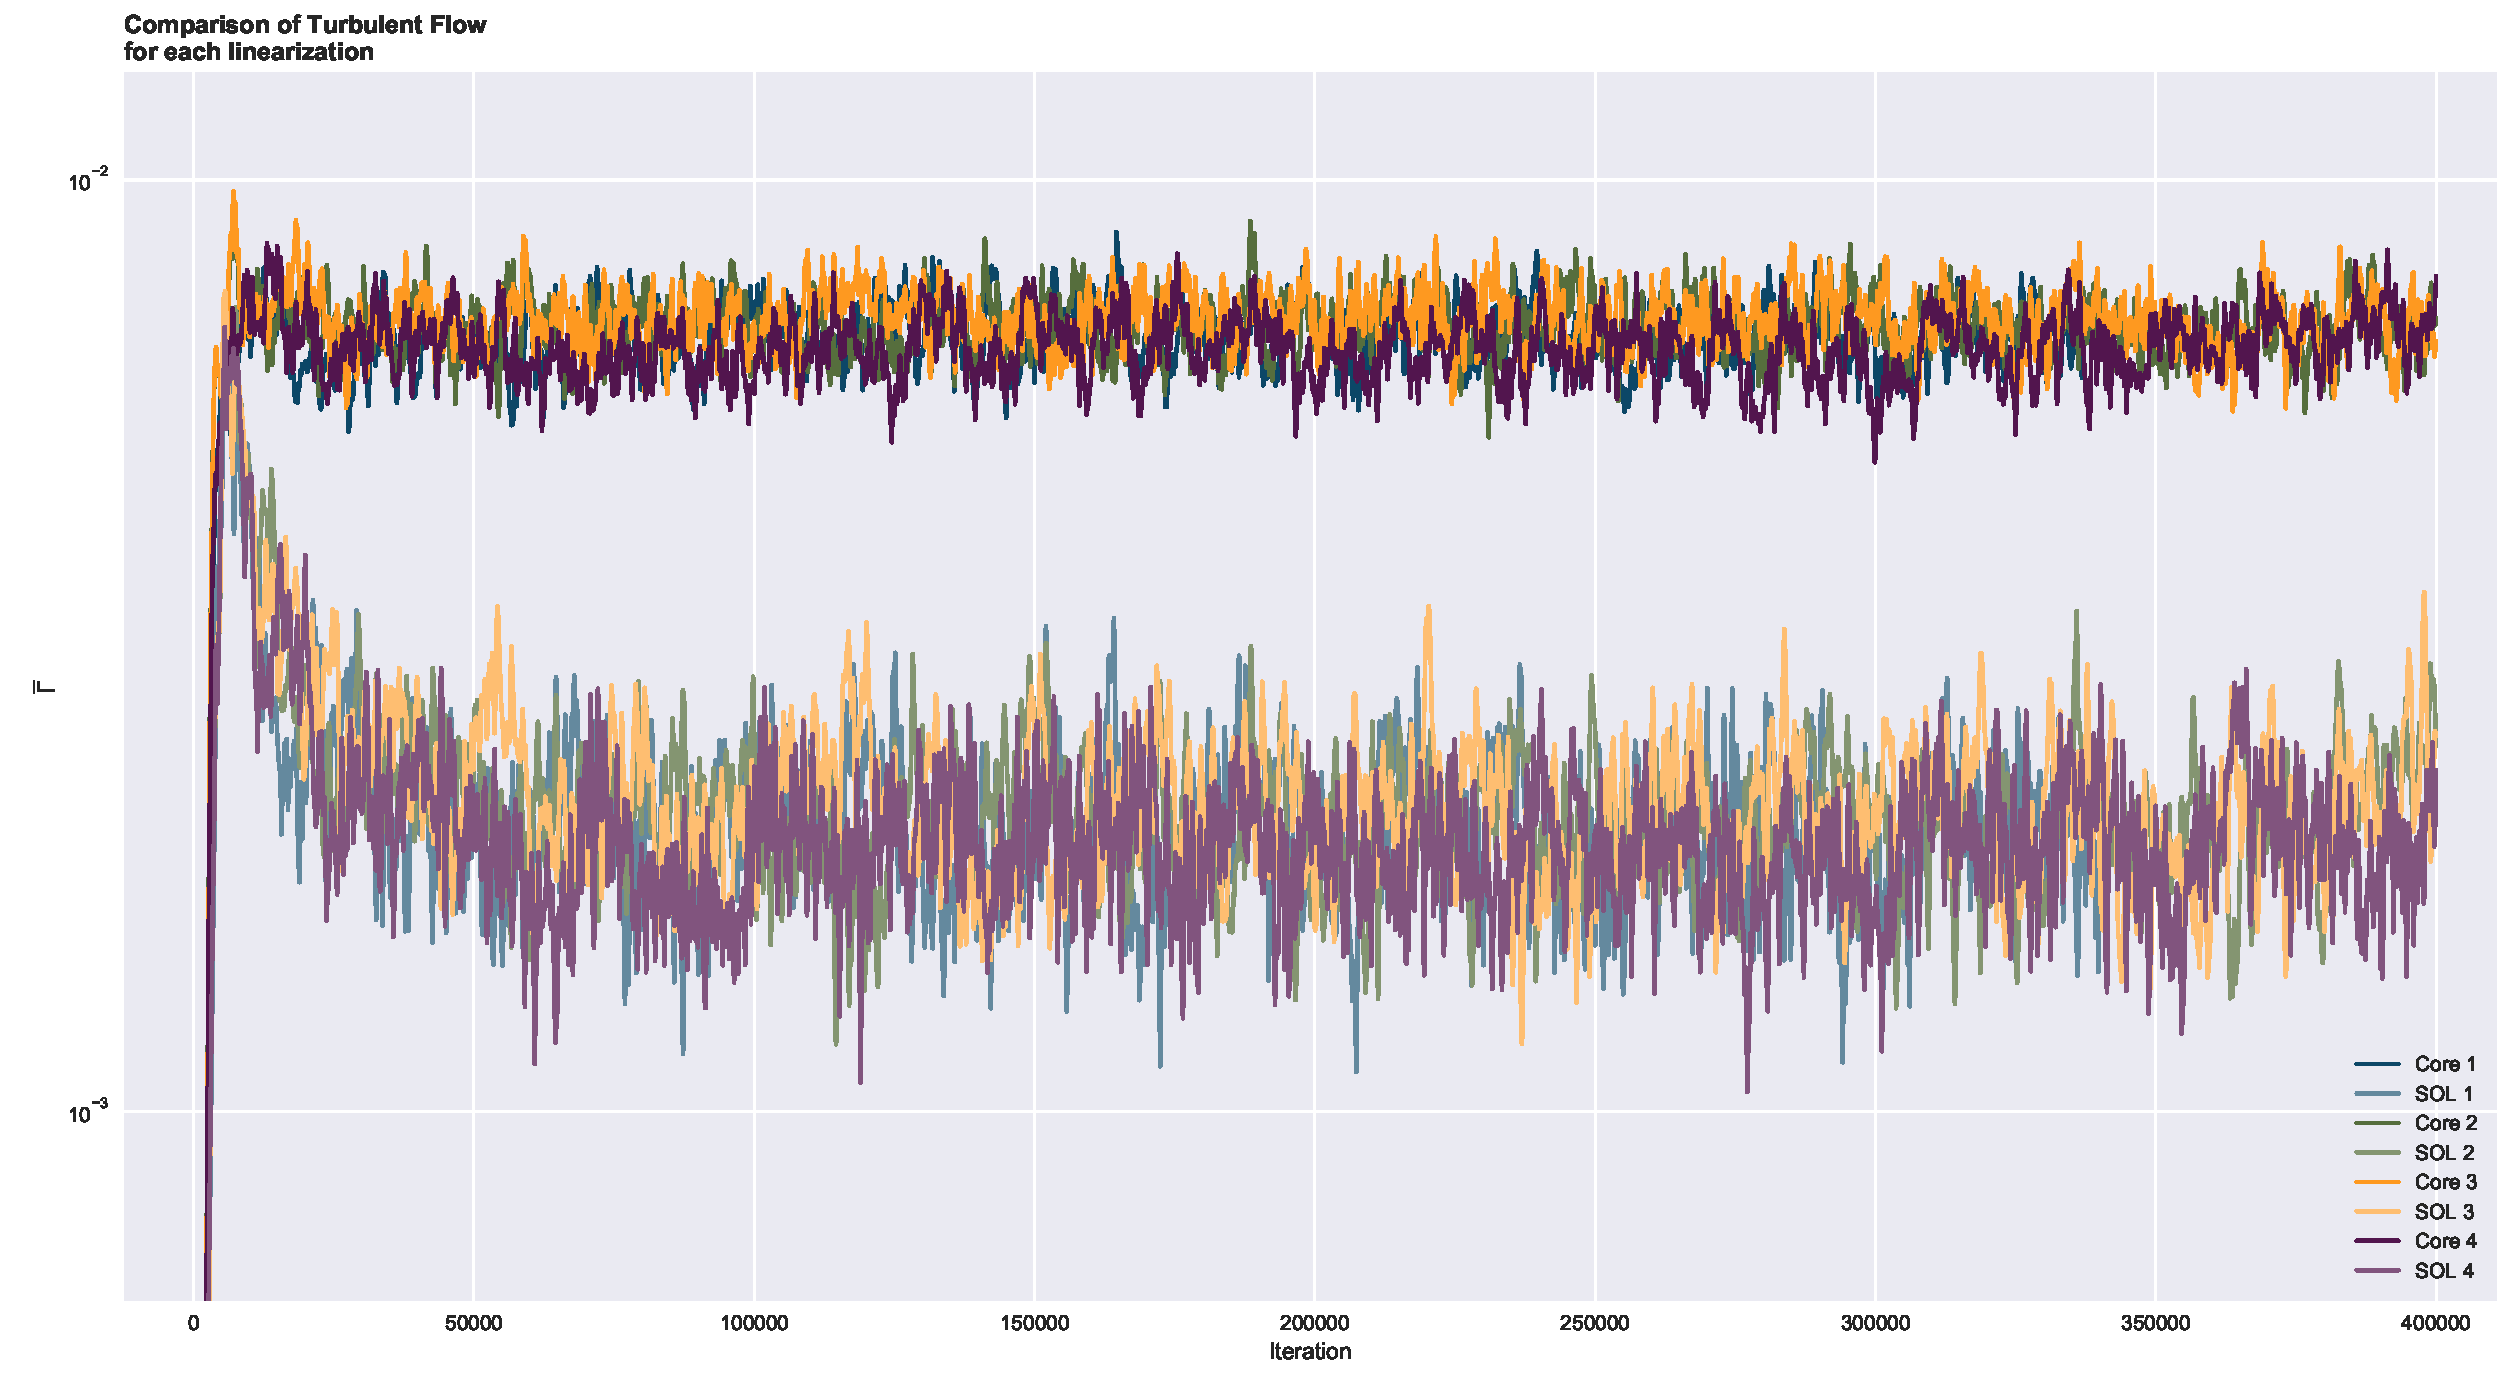
\includegraphics[width=\linewidth]{pdfs/turbulent-flow-low.pdf}
    \caption{Turbulent flow split into Core and \ac{SOL} region for each linearization. The lighter colors represent the \ac{SOL} parts.}
    \label{fig:turbulent-flow-low}
\end{figure}
\autoref{fig:turbulent-flow-low-means} shows the mean value of $\Tflow_{Core}$ and $\Tflow_{SOL}$ from 120,000 to 400,000 iterations. There may be a small indication that $\Tflow_{Core}$ is a little higher for the constant background (local model) lineraizations but considering the magnitude of fluctuations (visualized by the error bars) this seems very far fetched. 



\begin{figure}[!htbp]
    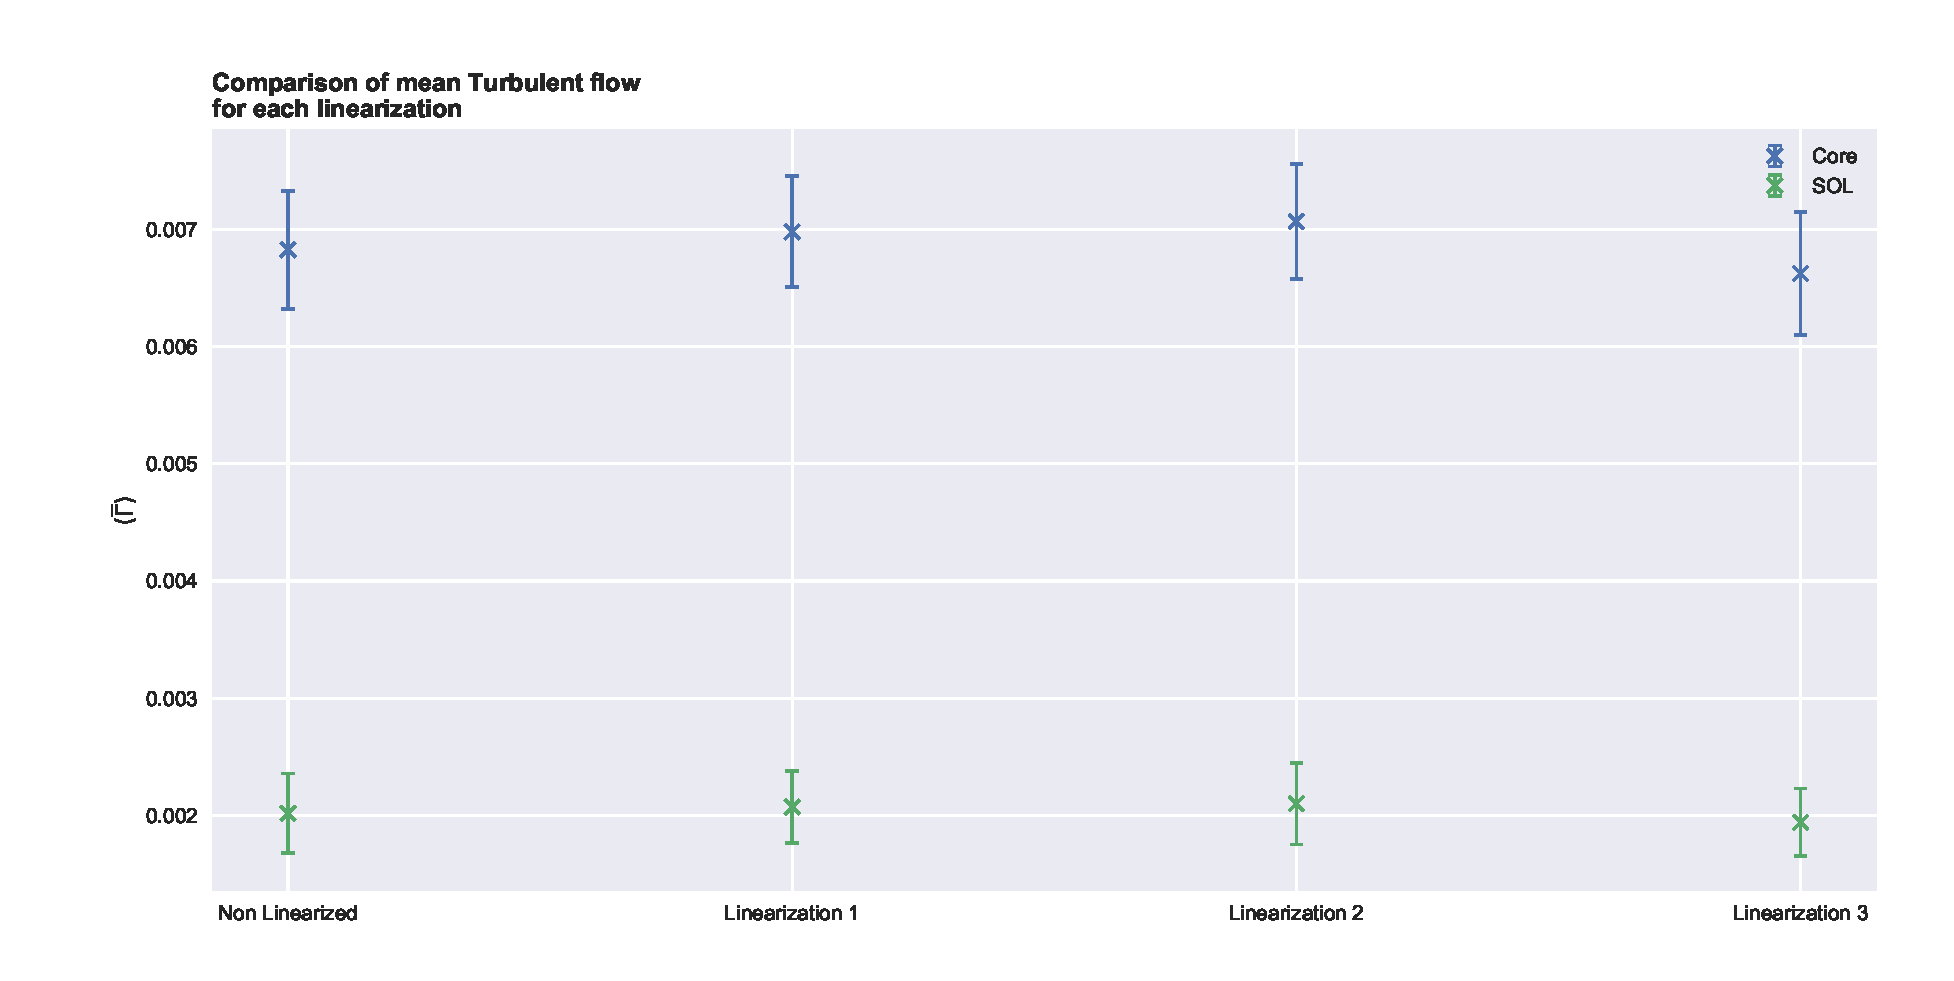
\includegraphics[width=\linewidth]{pdfs/turbulent-flow-low-means.pdf}
    \caption{Mean values of $\Tflow$ after 120,000 iterations. There is no apparent difference visible.}
    \label{fig:turbulent-flow-low-means}
\end{figure}

\section{Zonal Potential}

The same procedure of the previous section is applied to the zonal potential, zonal flow and zonal flow potential (vorticity). The results are shown in \autoref{fig:zonal-potential-low-all}.\\
The results form two groups: The non linearized model and the third linearization share distinct features as well as the first and the second. Since the linearization specifically targets the gradient of the densities which is the strongest close to the core plasma, the greatest difference between the linearizations and the non linearized model is observed there. One has to note that on the boundaries numerical artifacts play a major role leading to artificial density gradients of first and second order explaining for instance the \textit{bump} on the $x_L$ boundary.

\begin{figure}[!htbp]
    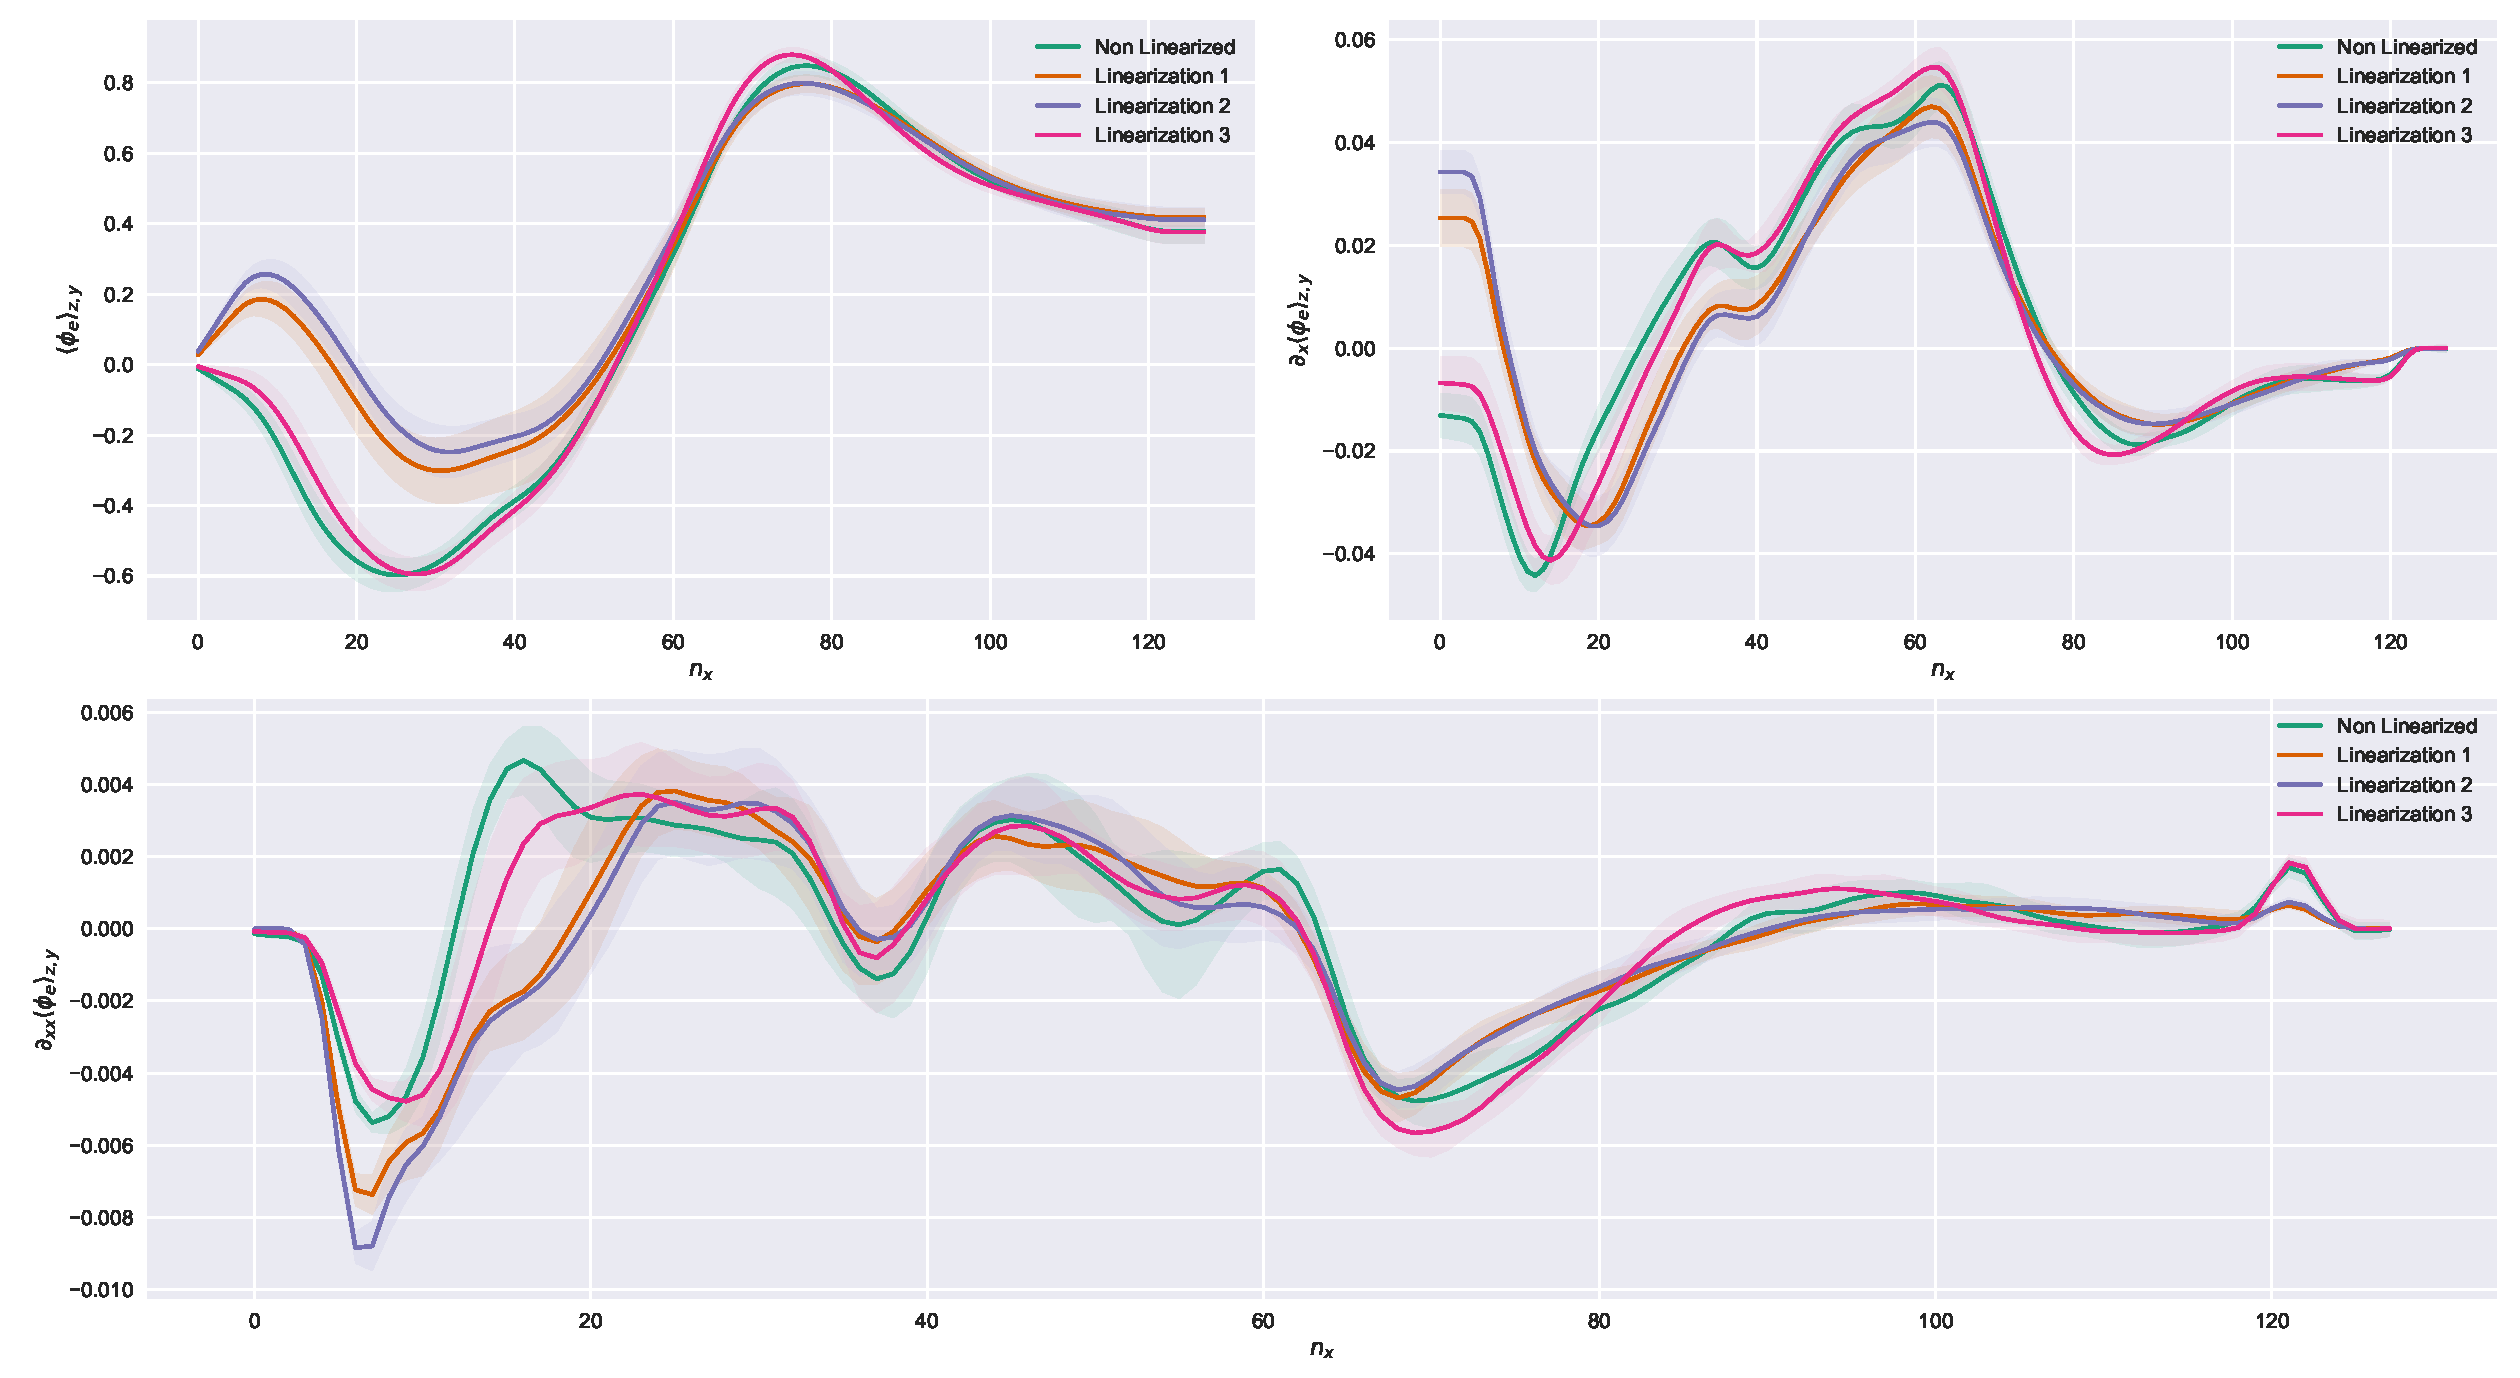
\includegraphics[width=\linewidth]{pdfs/zonal_potential_low.pdf}
    \caption{Mean values of Zonal Potential, Zonal Flow and Zonal Flow Potential of iteration 120,000-400,000}
    \label{fig:zonal-potential-low-all}
\end{figure}

\section{Parallel Velocities}

Another quantity can be defined as following:
\begin{equation}
    \mathrm{E}_{v_\parallel} = \hat{\epsilon} \cdot \int_{[z,x,y]} \left( \mu_ev_{e\parallel}^2 + \mu_iv_{i\parallel }^2 \right) \, dxdydz
\end{equation}
which essentially is the parallel kinetic energy of the system.
As in the previous chapters the integration will be restricted to either Core or the \ac{SOL} region. The time evolution of these quantities is shown in \autoref{fig:velocity-energy-low}.

\begin{figure}[!htbp]
    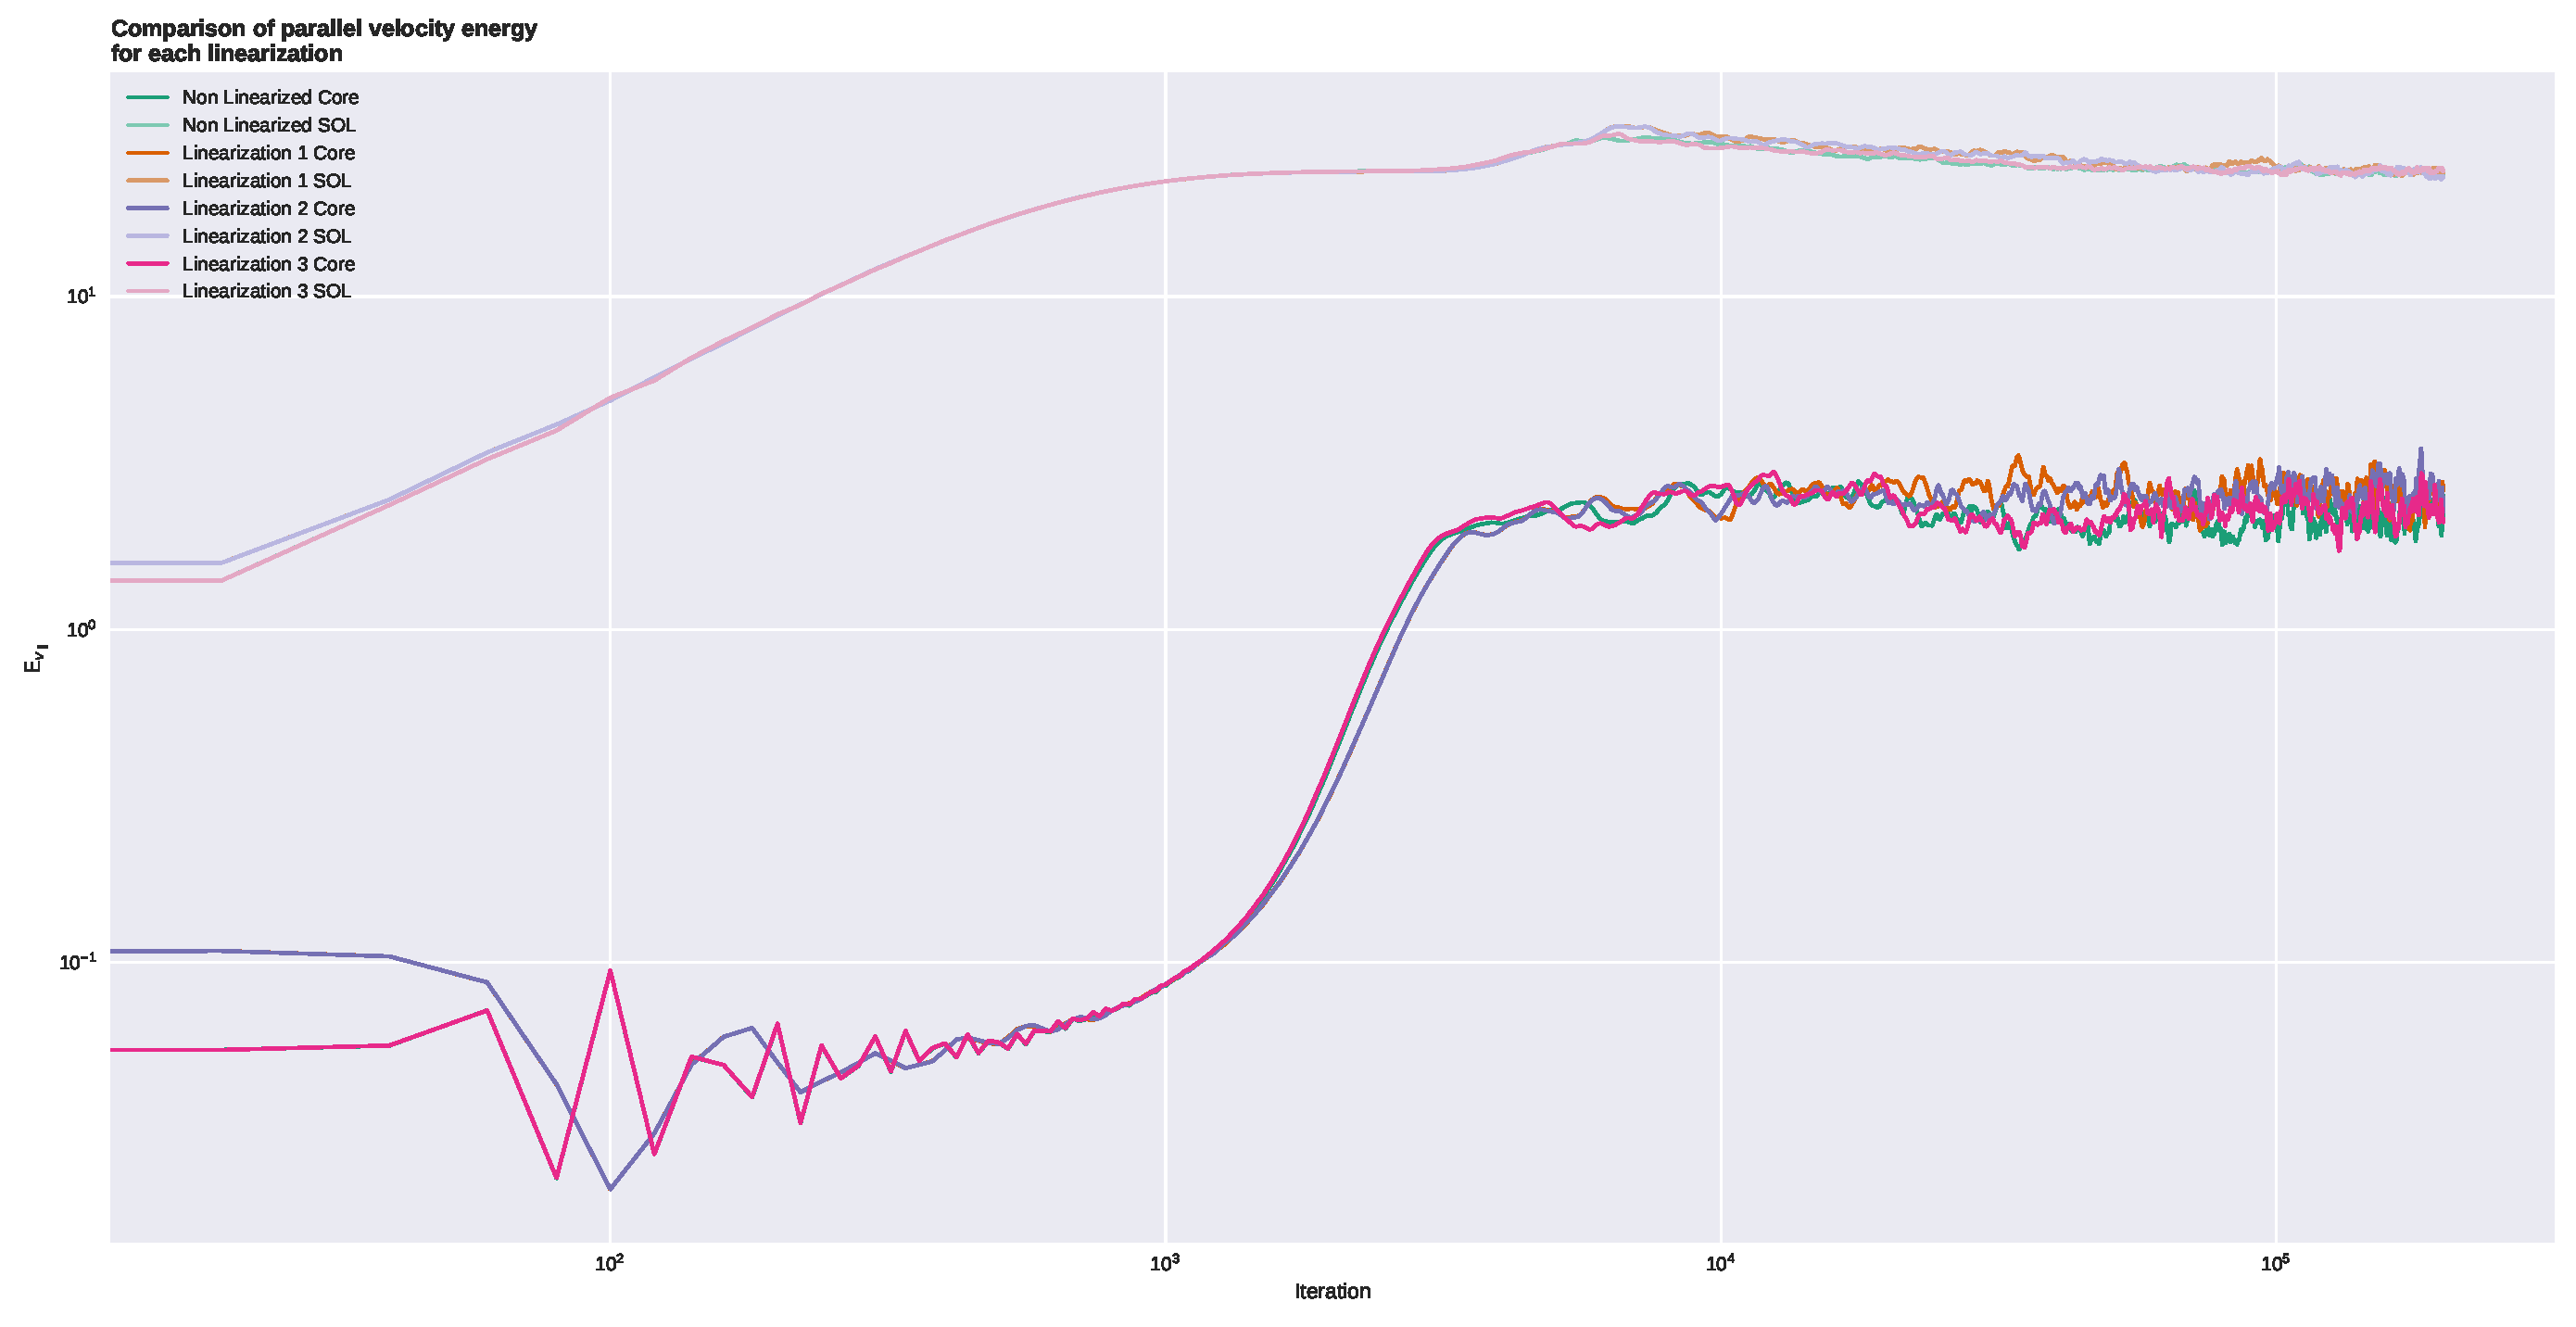
\includegraphics[width=\linewidth]{pdfs/velocity-energy-low.pdf}
    \caption{Time evolution of $\mathrm{E}_{v_\parallel}$ for Core and \ac{SOL} region}
    \label{fig:velocity-energy-low}
\end{figure}

The comparison shows no major difference but if one looks at the mean values the splitting into two groups from the previous section is visible again (\autoref{fig:velocity-energy-low-mean}).


\begin{figure}[!htbp]
    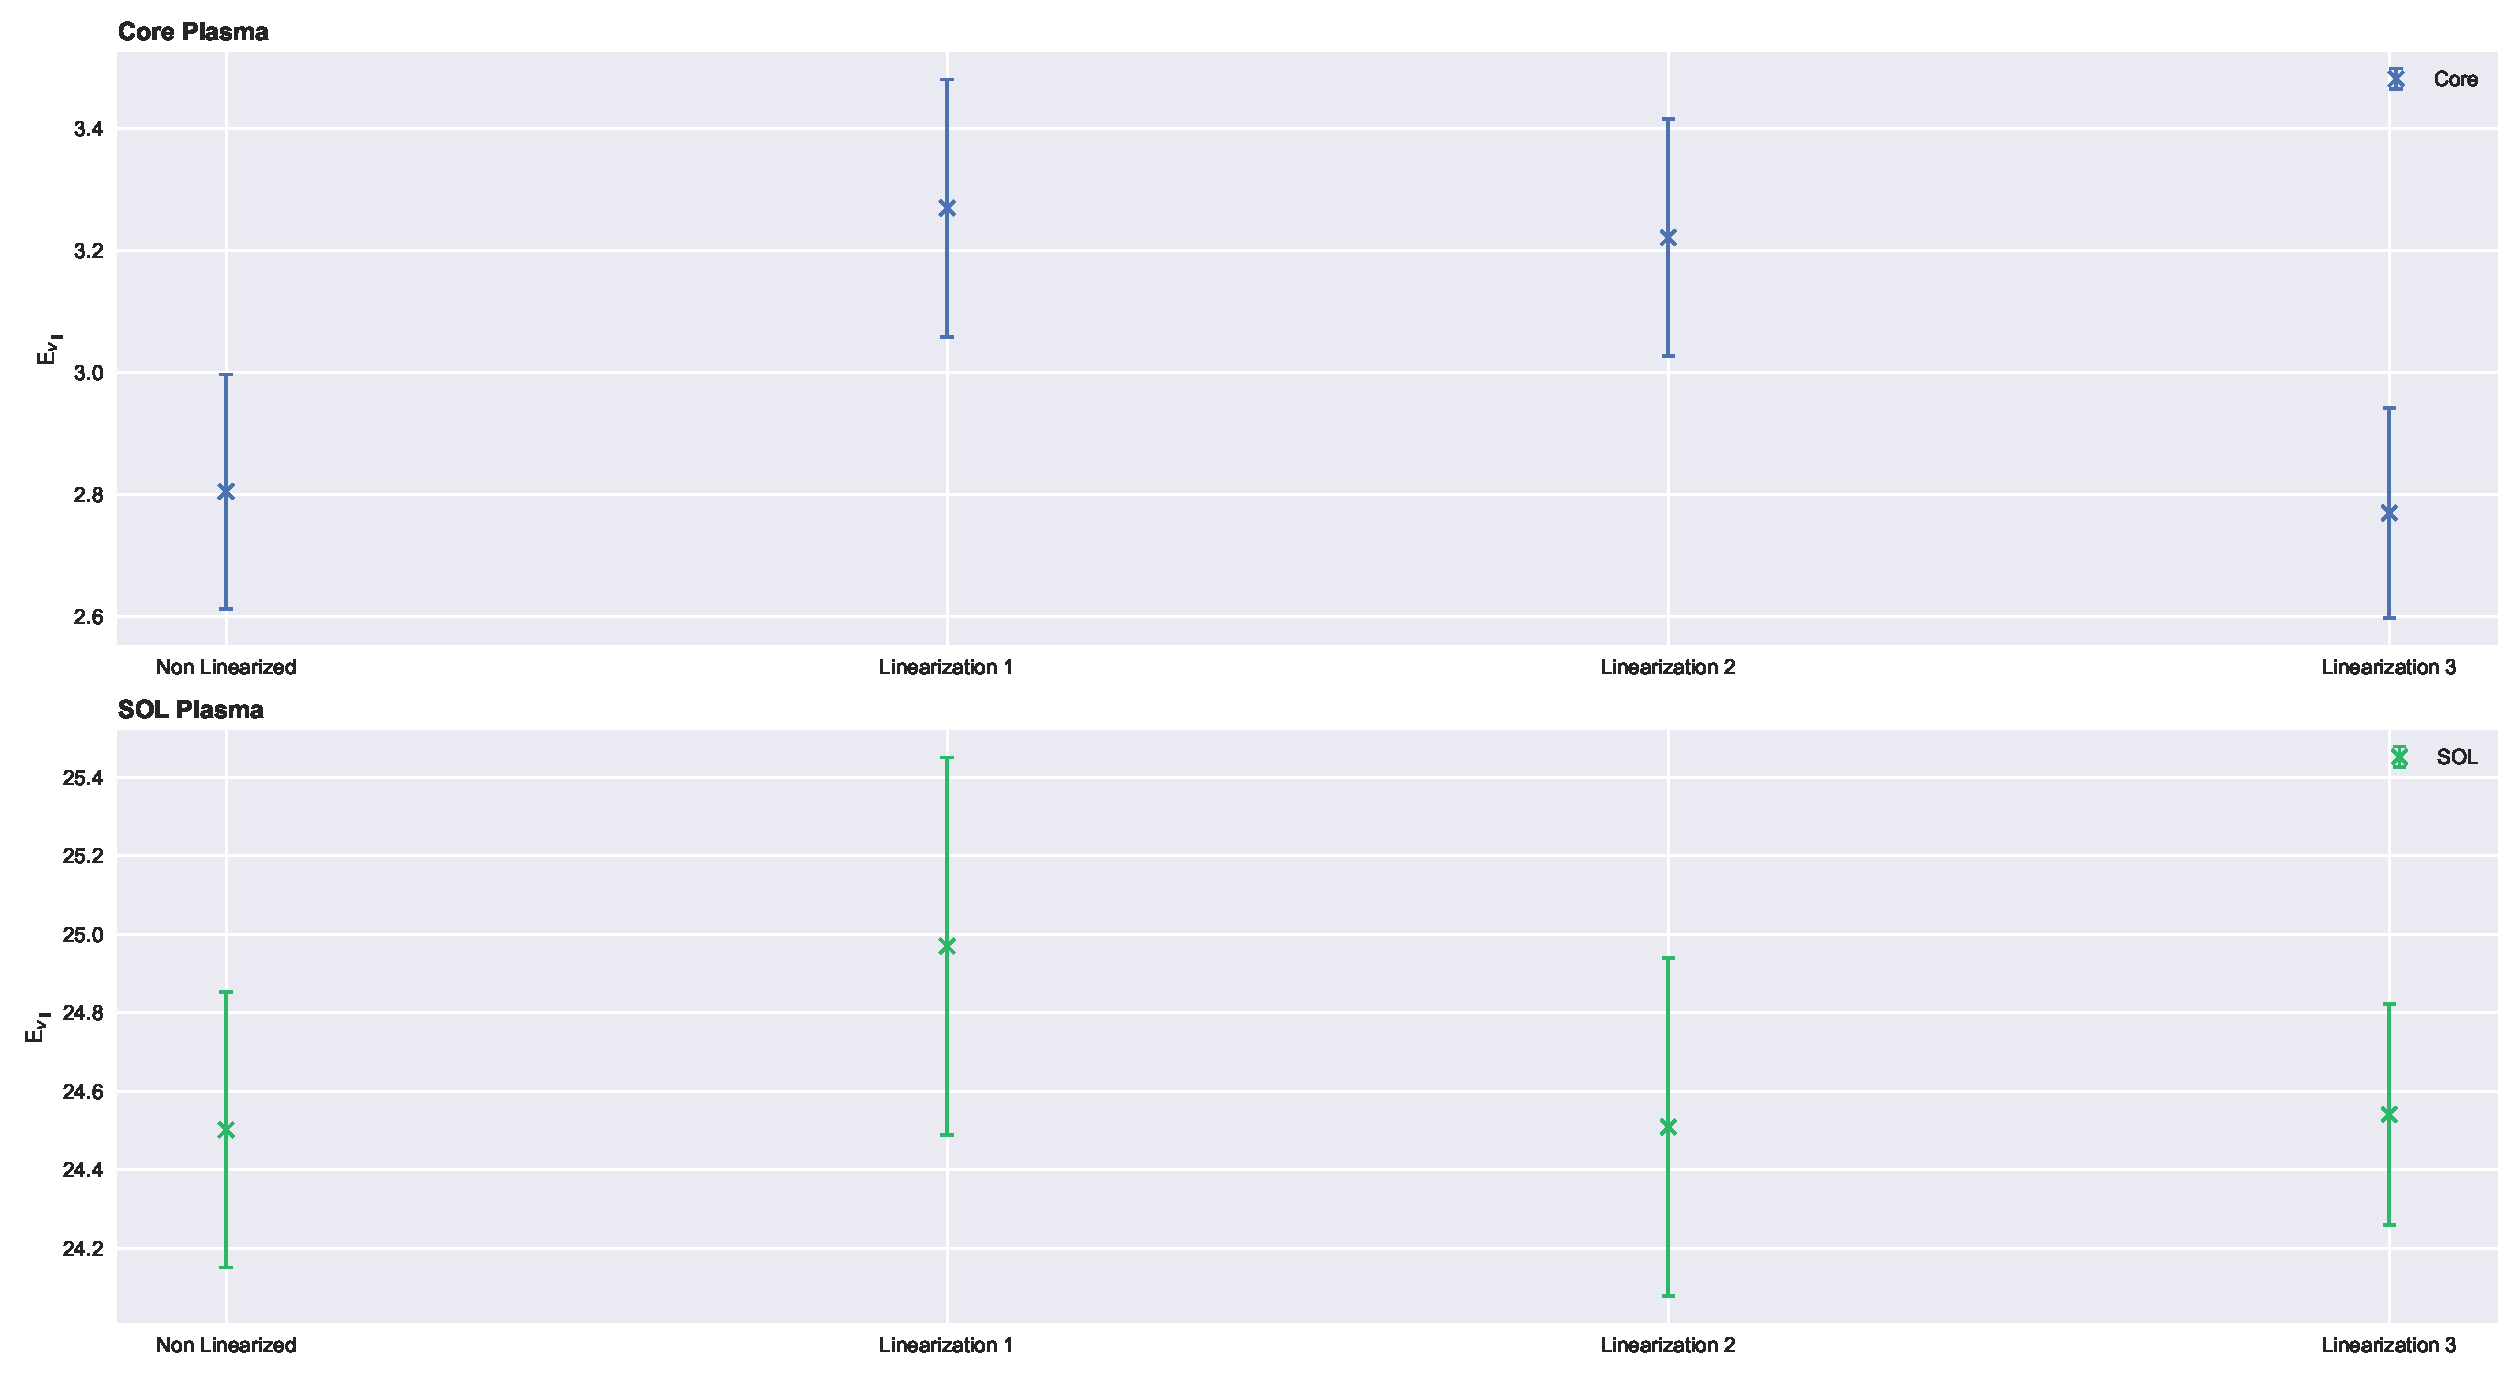
\includegraphics[width=\linewidth]{pdfs/velocity-energy-low-means.pdf}
    \caption{Mean of Velocity Energy from 120,000 to 400,000 iterations}
    \label{fig:velocity-energy-low-mean}
\end{figure}

\section{Numerical stability}
Not thoroughly measured was the stability of the simulation but still some information will be presented here. For example if one increases the magnetic curvature to 0.05 for the lower resolution grid (leading to stronger turbulence) only the non linearized model is numerical stable. One has to deal with high gradients at the boundaries which seem to be a greater problem for the linearized models. 
Furthermore if the resolution is increased the $\Delta t$ has to be decreased but the non linearized model is still stable for higher $\Delta t$'s whereas the linearizations are much more sensitive to an increase of the resolution and need smaller $\Delta t$'s. It seems that the \ac{CFL} limit is generally lower for the linearized models.




\end{document}